\part{Verschlüsselung Allgemein}
\section{Sinn und Zweck der Verschlüsselung}
Die Verschlüsselung bzw. die Geheimhaltung von Informationen gibt es schon lange. Die Frage ist, wie kann ich eine Information vor aussenstehende so darstellen dass es für sie keinen Sinn ergibt. Ich, oder andere, mit einem geheimen Schlüssel die Information lesen können. Im realen Leben können wir zum Beispiel unser Haus vor Dieben sichern, indem wir eine Türe mit einem stabilen Schloss einbauen. Möchte man noch weiter gehen, kann man eine Alarmanlage einabauen.\\[2ex]
%
In der Digitalen Welt geht das nicht so einfach. Obwohl man seinen Rechner mit einem Benutzername und Passwort für unbefugte Personen schützen kann, gibt es Techniken, mit der lassen sich ganze Festplatten Bit für Bit kopieren. Hier setzt die Verschlüsselung an. Denn wenn man etwas verschlüsselt auf die Festplatte speichert, kann der unbefugte die gestohlenen Daten nicht brauchen.
\section{Geschichte der Verschlüsselung}
\subsection{Klassische Kryptografie}
Die Kryptographie bezeichnet die Entwicklung von Methoden zur Verheimlichung von Nachrichten.
Solche Methoden wurden schon 3000 Jahre vor Christus bei den Ägyptern verwendet(Hyrogliphen). \\
Die Hebräer haben 600 vor Christus das Atbash entwickelt. Dabei wurde das Alphabet umgekehrt und entsprechend verschlüsselt.
Als kleines Beispiel

\begin{table}[ht]
\caption{Atbash Verschlüsselung}
\begin{center}
\begin{tabular}{|l|l|l|l|l|l|l|}
  a & b & c & d & e & f\\
  z & y & x & w & v & u\\
\end{tabular}
\end{center}
\end{table}


Die Caesar-Verschlüsselung wurde nach Julius Caesar benannt und zur militärischen Korrespondenz im Römischen Reich gebraucht.\\
Dafür wurde damals das Alphabet um 3 Stellen nach hinten verschoben. Aus einem D wird somit ein A. Dieses Verfahren wurde im 15.-Jahrhundert mit einer
Chiffrierscheibe verbessert und ist bis heute noch als Caesar Verschlüsselung bekannt. Die Verschiebung um 13 Stellen wird auch als Rot13 bezeichnet, 
da das Alphabet aus 26 Zeichen besteht, ist die Verschlüsselung und Entschlüsselung bei Rot13 die selbe.

\begin{table}[ht]
\caption{Caesar Verschlüsselung um 3 Zeichen}
\begin{center}
\begin{tabular}{|l|l|l|l|l|l|l|}
  a & b & c & d & e & f\\
  x & y & z & a & b & c\\
\end{tabular}
\end{center}
\end{table}

All diese Verfahren können ziemlich eifach geknackt werden. Da bestimmte Buchstaben in einer Sprache öfter vorkommen, kann durch Textanalyse die Verschiebung herausgefunden werden. Ebenfalls wird der Grundsatz verletzt, dass die Sicherheit nicht von der Geheimhaltung
des Algorythmus abhängen 

\subsection{Kryptographie im zweiten Weltkrieg}
Im zweiten Weltkrieg nutzten die Deutsche Wehrmacht die ENIGMA zur Verschlüsselung ihres Funkverkehrs. Die ENIGMA ist wie eine Schreibmaschine zu bedienen. Die ENIGMA besteht aus der Tastatur, einem Walzensatz und einer Anzeige über Lampen. 

\begin{figure}[ht]
\begin{center}
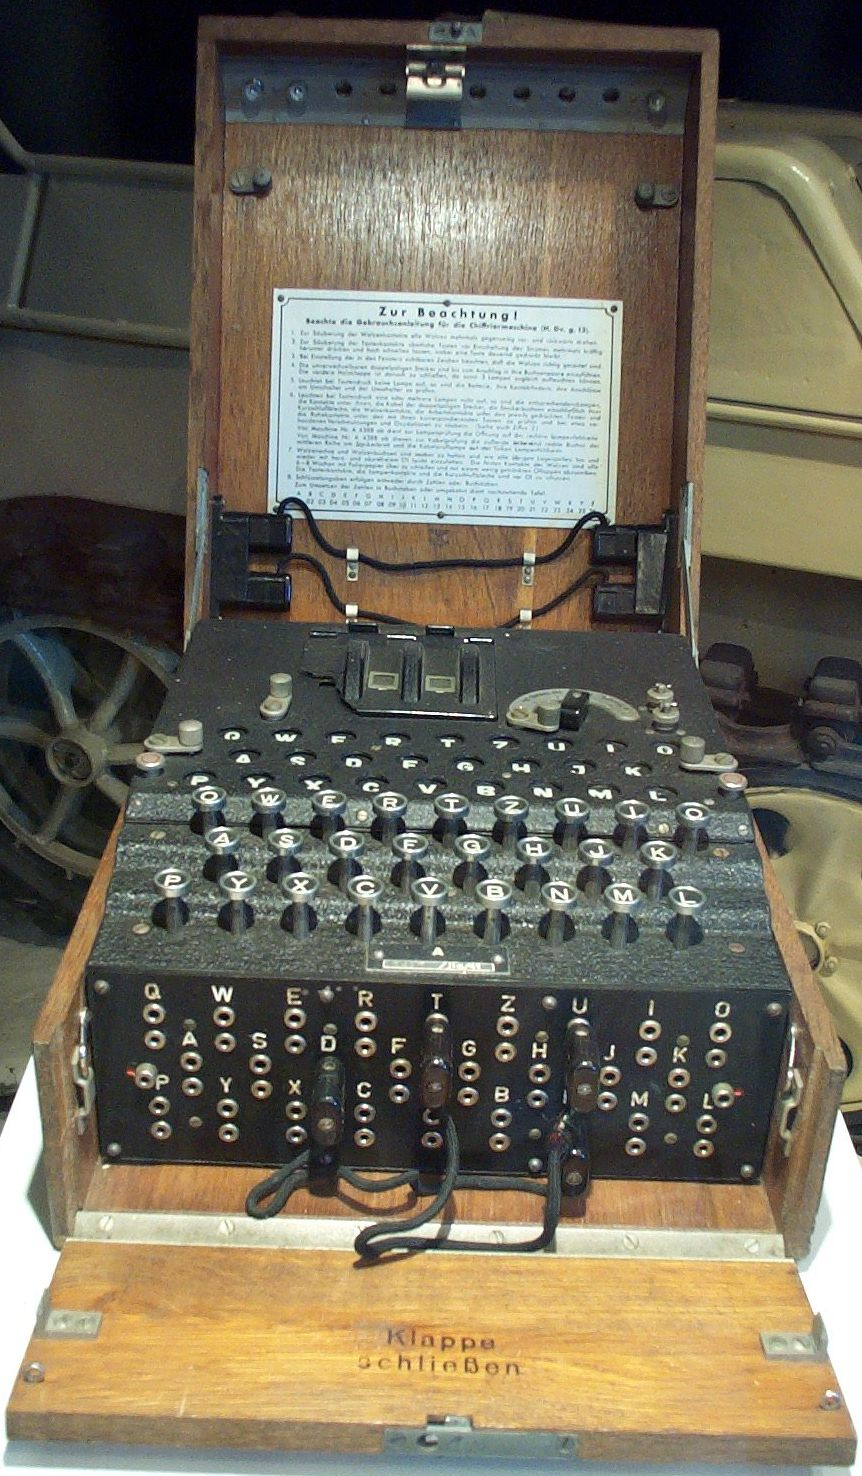
\includegraphics[width=5cm]{images/Enigma_Verkehrshaus_Luzern_cropped.jpg}
\caption{Enigma Maschine}
\end{center}
\end{figure}

\subsubsection{Funktion der ENIGMA Maschine}
Die Walzen können sich drehen und sind mit Elektrischen Kontakten miteinander verbunden. Wird eine Taste gedrückt, fliesst Strom durch den Walzenssatz und es leuchtet die Lampe des verschlüsselten Buchstabens auf. Die Walze dreht sich bei jedem Tastendruck weiter, so das der gleiche Buchstaben jeweils anders verschlüsselt wird. Z. B. AAA wird zu DEF. Nach 26 Umdrehungen der ersten Walze wird die zweite Walze gedreht. \\

\begin{figure}[ht]
\begin{center}
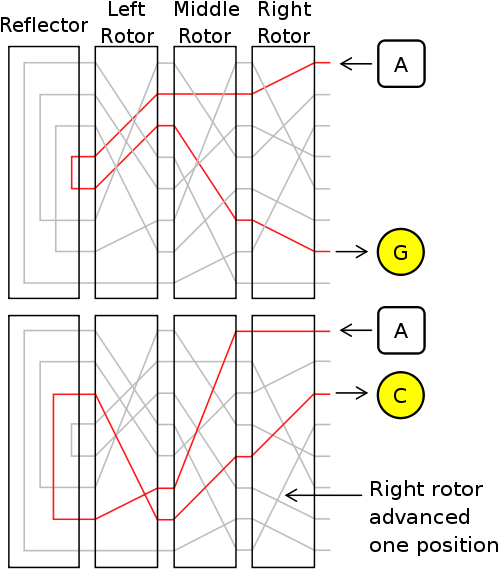
\includegraphics[width=5cm]{images/Enigma-action.png}
\caption{Enigma Stromfluss}
\end{center}
\end{figure}

Dabei gehen jeweils elektrische Impulse durch die Walze. Nach jeder Drehung legt der Strom eine andere Strecke durch die Walzen zurück. 
Über das Steckbrett konnte der Verschlüsselte Buchstaben nochmals ersetzt werden. z. B. wurde E mit J verbunden. Falls nach dem verschlüsseln ein E herauskam, wurde dieses mit J ersetzt. 

\subsubsection{Anwendung}
Die Deutsche Wehrmacht nutzte die ENIGMA um ihre Funksprüche zu verschlüsseln. Dazu wurden jeweils um Mitternacht die Walzen und die Steckverbindungen ausgetauscht bzw. umgesteckt. Ein neuer Schlüsselsatz sah beispielsweise so aus:

%Quelle Wikipedia%
\begin{table}[ht]
\caption{Schlüsseltafel der Wehrmacht}
\begin{center}
\begin{tabular}{|l|l|l|l|l}
Tag & UKW & Walzenlage & Ringstellung &  ---- Steckerverbindungen ---- \\
 31  &   B   &  I   IV III   &    16 26 08   &  AD CN ET FL GI JV KZ PU QY WX \\
\end{tabular}
\end{center}
\end{table}

Die eigentliche Verschlüsselung war relativ simpel zu bewerkstelligen. Es musste nur die entsprechende Funknachricht eingegeben werden und die ENIGMA erledigte die Verschlüsselung. Der Austausch der aktuellen Walzenstellung und das Morsen der Nachricht waren jedoch wesentlich komplizierter.

Vor der Eigentlichen Nachricht wurde ein Nachrichtenkopf gemorst. In diesem wurde die länge des Textes bekannt gegeben, die Walzenstellung und die Nachrichtenart. 
Der eigentliche Text wurde in Gruppen aus 5 Buchstaben gemorst. Bei den ersten 5 Buchstaben wurde bestimmt, an wenn die Nachricht geht. Dabei wurden die ersten zwei Buchstaben zufällig ausgewählt und die letzten 3 durchmischt. Nach der Alphabetischen Ordnung, konnte über eine Tabelle festgestellt werden, ob die Nachricht einem was angeht, bevor man sie entschlüsselt.
Die Walzenstellung wurde ebenfalls nicht einfach übertragen. Wenn im Kopf z. B. QWE EWG angegeben wurde, hiess das man soll die Walze auf die Buchstaben QWE einstellen und EWG eingeben. Was dabei verschlüsselt heraus kam, war die Anfangsstellung der Walzen. Jetzt konnte mit der Decodierung der Nachricht begonnen werden.

\subsubsection{Schwachstelle der ENIGMA}
Die Enigma benutzte ein Symetrisches Verfahren, wobei die Verschlüsselung und Entschlüsselung gleich sind. %Siehe Kapitel Symetrische Verfahren%
Die Geheimhaltung der Walzen war wichtig, da sie einen wesentlichen Teil der Verschlüsselung ausmachen.
Dadurch das ein Buchstabe nicht in sich selbst verschlüsselt werden kann (Strom kann nicht zurück fliessen) konnte ein wesentlicher Teil ausgeschlossen werden.
Durch einsetzen bestimmter Wörter, welche im Text vermutet wurden, konnte ein grosser Teil der möglichen Positionen ausgeschlossen werden. Dafür wurde z. B. OBERKOMMANDODERWEHRMACHT eingesetzt und falls an einer Position der Buchstabe in sich selbst verschlüsselt war, konnte das Wort an dieser Position nicht sein.

\subsection{Probleme der früheren Verschlüsselungen}
Die Verfahren bis zum zweiten Weltkrieg konnten einfach geknackt werden. Wenn die Art der Verschlüsselung bekannt war, konnte der Schlüssel einfach ermittelt werden. 
Die Enigma revolutionierte die Kryptographie. Obwohl die Art der Verschlüsselung und sogar die Walzen bekannt waren, mussten die Engländer grosse Anstrengungen unternehmen, damit die Texte entschlüsselt werden konnten. Um der Enigma zu begegnen wurden Maschinen gebaut, welche diese Arbeit vereinfachten. Die sogannte Turing Bombe konnte 


